\begin{figure}[ht]
\begin{center}
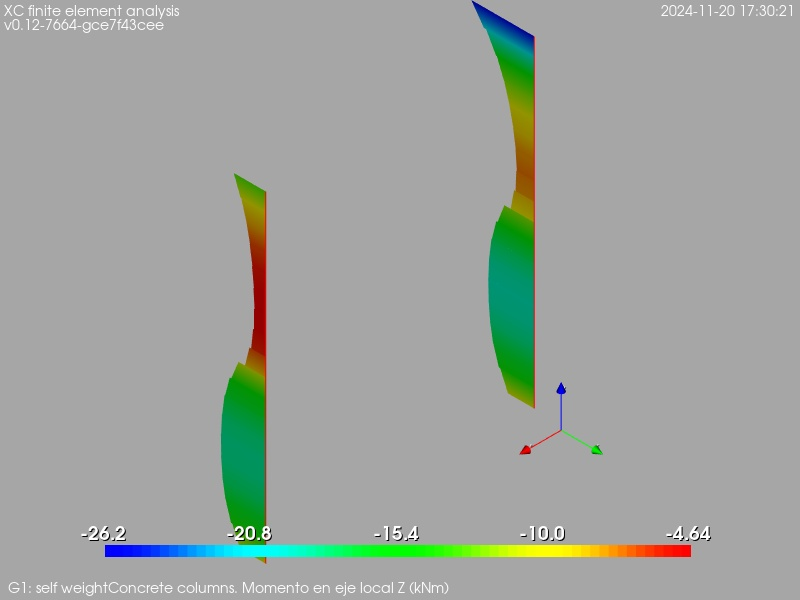
\includegraphics[width=\linewidth]{results/graphics/resSimplLC/GselfWeightcolumnZconcrMz.png}
\caption{ G1: self weightConcrete columns. Momento en eje local Z (kNm)}
\label{GselfWeightcolumnZconcrMz}
\end{center}
\end{figure}
\begin{figure}[ht]
\begin{center}
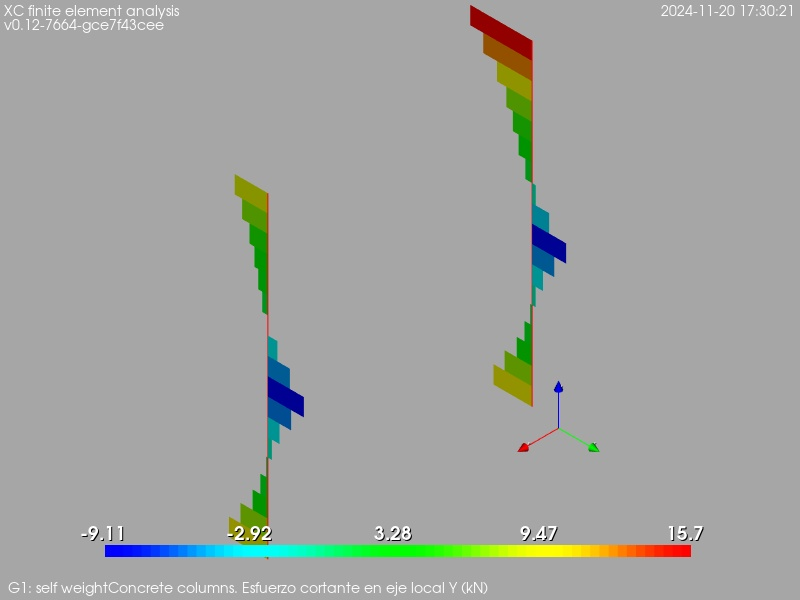
\includegraphics[width=\linewidth]{results/graphics/resSimplLC/GselfWeightcolumnZconcrVy.png}
\caption{ G1: self weightConcrete columns. Esfuerzo cortante en eje local Y (kN)}
\label{GselfWeightcolumnZconcrVy}
\end{center}
\end{figure}
\begin{figure}[ht]
\begin{center}
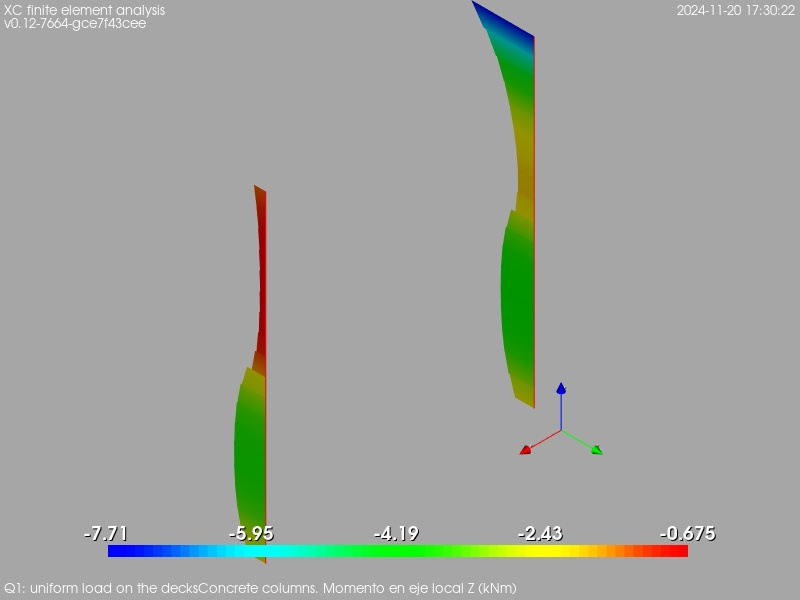
\includegraphics[width=\linewidth]{results/graphics/resSimplLC/QdeckscolumnZconcrMz.png}
\caption{Q1: uniform load on the decksConcrete columns. Momento en eje local Z (kNm)}
\label{QdeckscolumnZconcrMz}
\end{center}
\end{figure}
\begin{figure}[ht]
\begin{center}
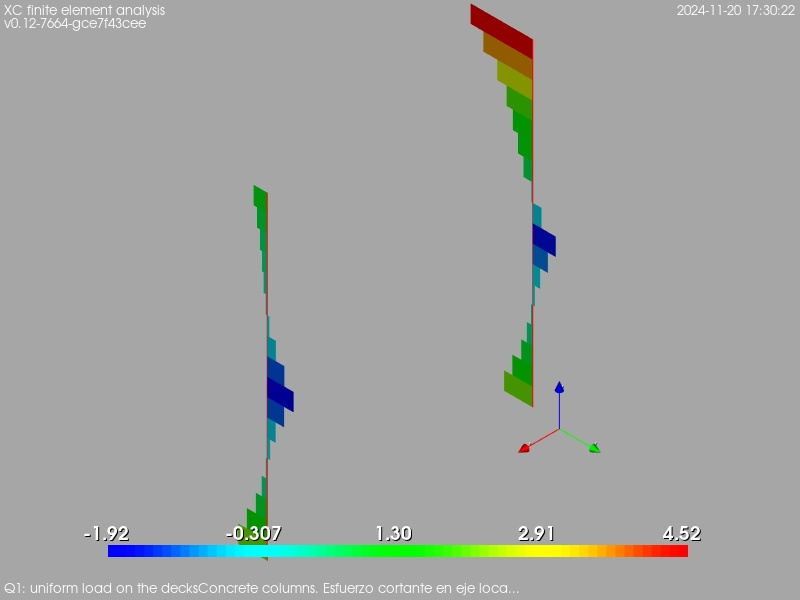
\includegraphics[width=\linewidth]{results/graphics/resSimplLC/QdeckscolumnZconcrVy.png}
\caption{Q1: uniform load on the decksConcrete columns. Esfuerzo cortante en eje local Y (kN)}
\label{QdeckscolumnZconcrVy}
\end{center}
\end{figure}
\begin{figure}[ht]
\begin{center}
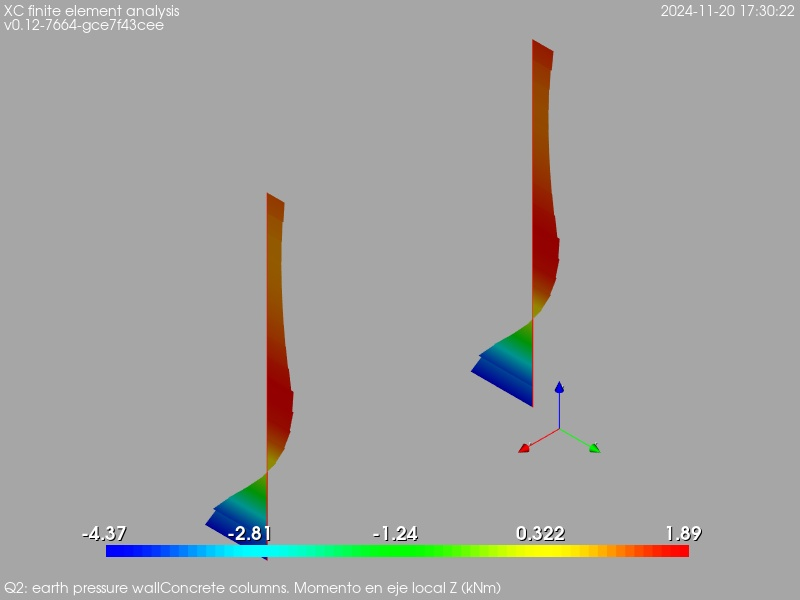
\includegraphics[width=\linewidth]{results/graphics/resSimplLC/QearthPressWallcolumnZconcrMz.png}
\caption{Q2: earth pressure wallConcrete columns. Momento en eje local Z (kNm)}
\label{QearthPressWallcolumnZconcrMz}
\end{center}
\end{figure}
\begin{figure}[ht]
\begin{center}
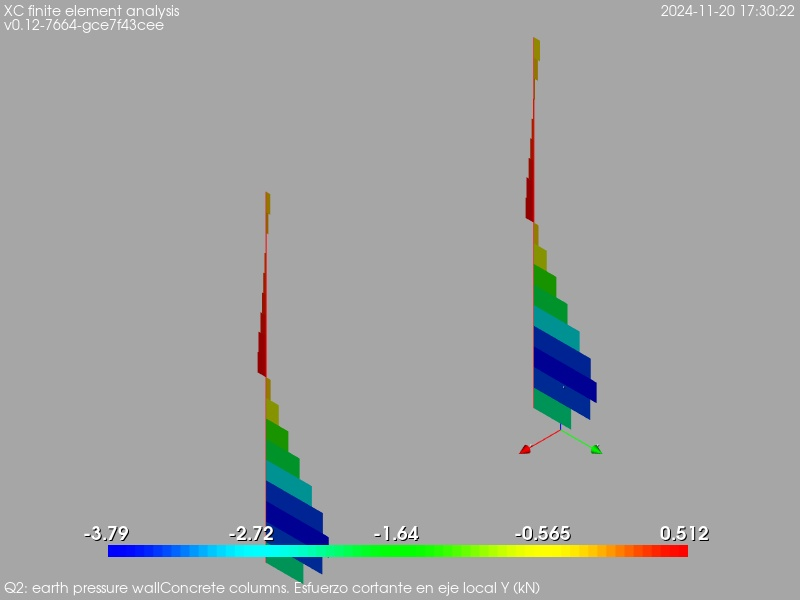
\includegraphics[width=\linewidth]{results/graphics/resSimplLC/QearthPressWallcolumnZconcrVy.png}
\caption{Q2: earth pressure wallConcrete columns. Esfuerzo cortante en eje local Y (kN)}
\label{QearthPressWallcolumnZconcrVy}
\end{center}
\end{figure}
\begin{figure}[ht]
\begin{center}
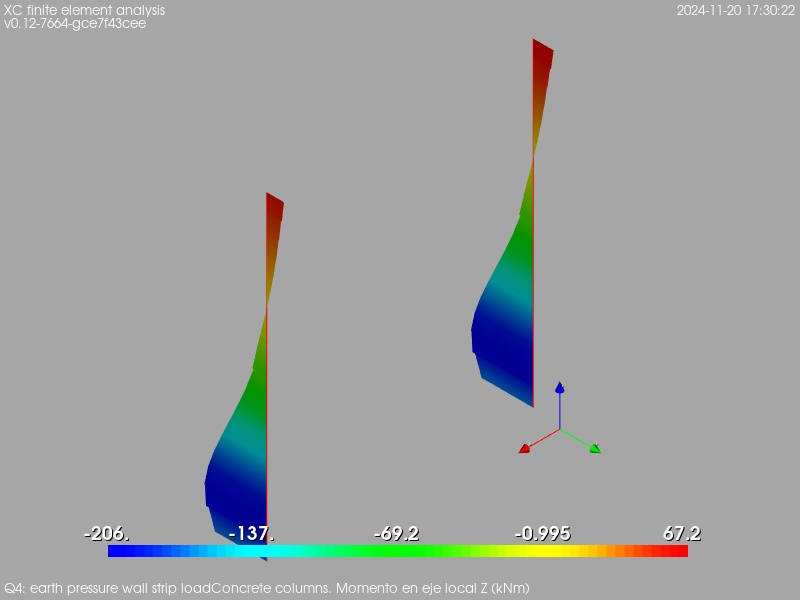
\includegraphics[width=\linewidth]{results/graphics/resSimplLC/QearthPWallStrLcolumnZconcrMz.png}
\caption{Q4: earth pressure wall strip loadConcrete columns. Momento en eje local Z (kNm)}
\label{QearthPWallStrLcolumnZconcrMz}
\end{center}
\end{figure}
\begin{figure}[ht]
\begin{center}
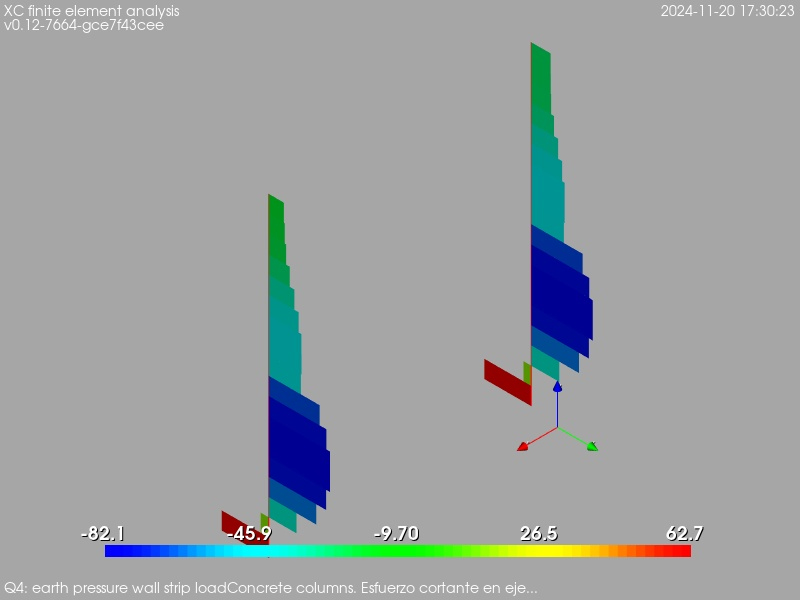
\includegraphics[width=\linewidth]{results/graphics/resSimplLC/QearthPWallStrLcolumnZconcrVy.png}
\caption{Q4: earth pressure wall strip loadConcrete columns. Esfuerzo cortante en eje local Y (kN)}
\label{QearthPWallStrLcolumnZconcrVy}
\end{center}
\end{figure}
\begin{figure}[ht]
\begin{center}
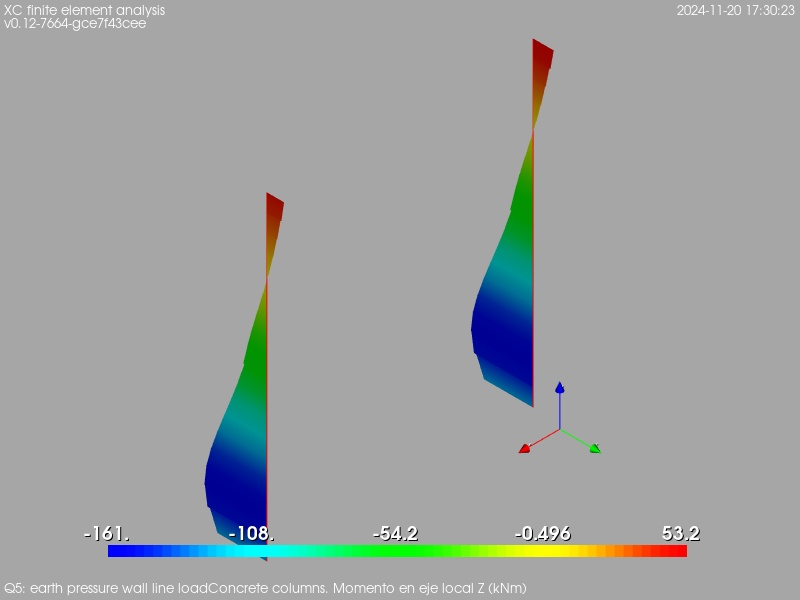
\includegraphics[width=\linewidth]{results/graphics/resSimplLC/QearthPWallLinLcolumnZconcrMz.png}
\caption{Q5: earth pressure wall line loadConcrete columns. Momento en eje local Z (kNm)}
\label{QearthPWallLinLcolumnZconcrMz}
\end{center}
\end{figure}
\begin{figure}[ht]
\begin{center}
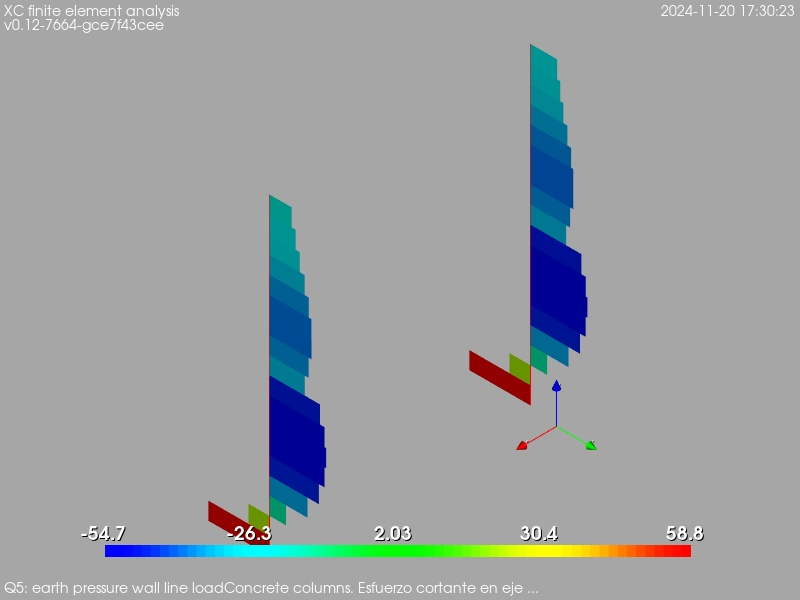
\includegraphics[width=\linewidth]{results/graphics/resSimplLC/QearthPWallLinLcolumnZconcrVy.png}
\caption{Q5: earth pressure wall line loadConcrete columns. Esfuerzo cortante en eje local Y (kN)}
\label{QearthPWallLinLcolumnZconcrVy}
\end{center}
\end{figure}
\begin{figure}[ht]
\begin{center}
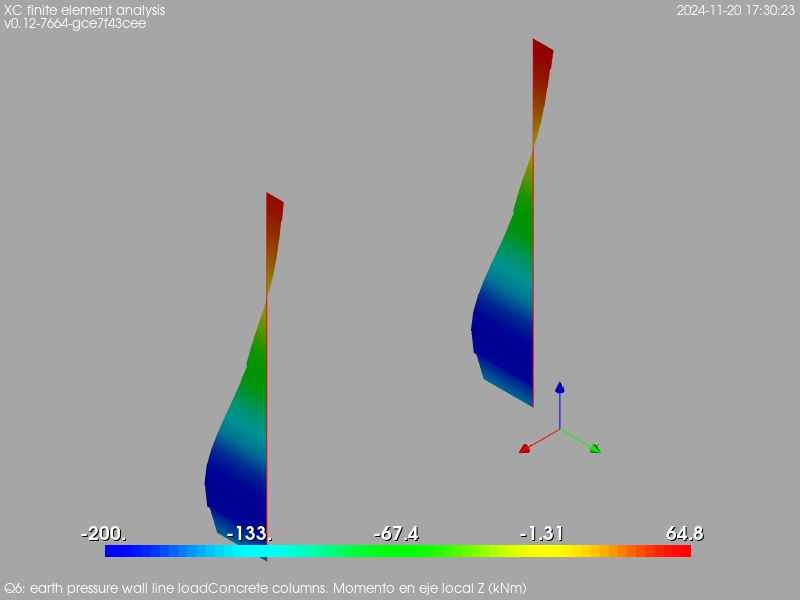
\includegraphics[width=\linewidth]{results/graphics/resSimplLC/QearthPWallHrzLcolumnZconcrMz.png}
\caption{Q6: earth pressure wall line loadConcrete columns. Momento en eje local Z (kNm)}
\label{QearthPWallHrzLcolumnZconcrMz}
\end{center}
\end{figure}
\begin{figure}[ht]
\begin{center}
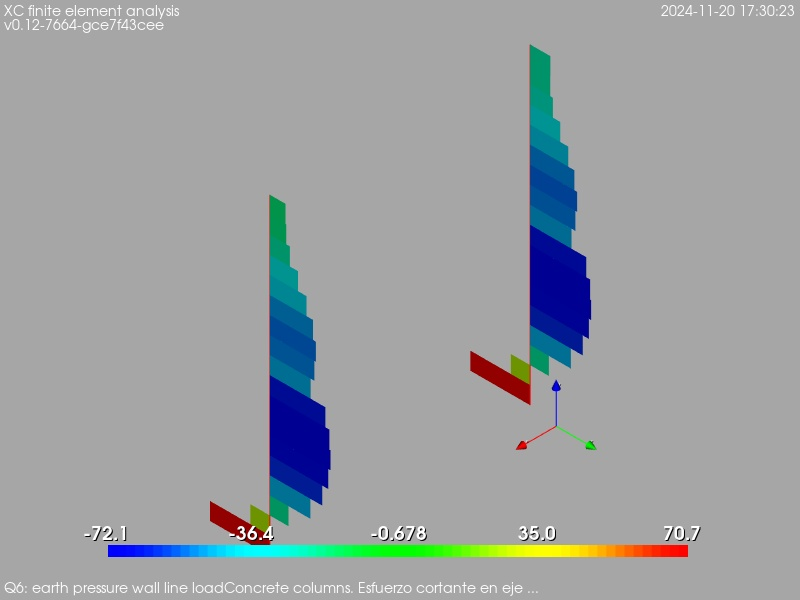
\includegraphics[width=\linewidth]{results/graphics/resSimplLC/QearthPWallHrzLcolumnZconcrVy.png}
\caption{Q6: earth pressure wall line loadConcrete columns. Esfuerzo cortante en eje local Y (kN)}
\label{QearthPWallHrzLcolumnZconcrVy}
\end{center}
\end{figure}
\begin{figure}[ht]
\begin{center}
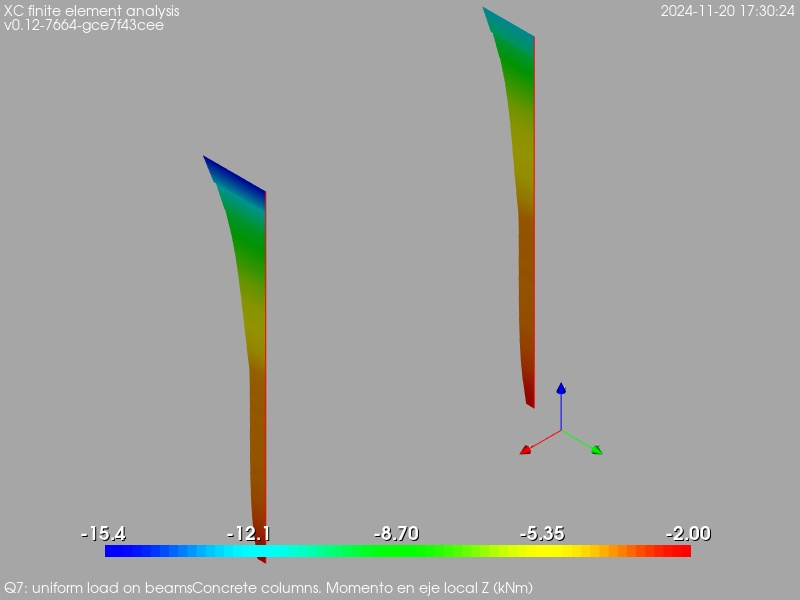
\includegraphics[width=\linewidth]{results/graphics/resSimplLC/qunifBeamscolumnZconcrMz.png}
\caption{Q7: uniform load on beamsConcrete columns. Momento en eje local Z (kNm)}
\label{qunifBeamscolumnZconcrMz}
\end{center}
\end{figure}
\begin{figure}[ht]
\begin{center}
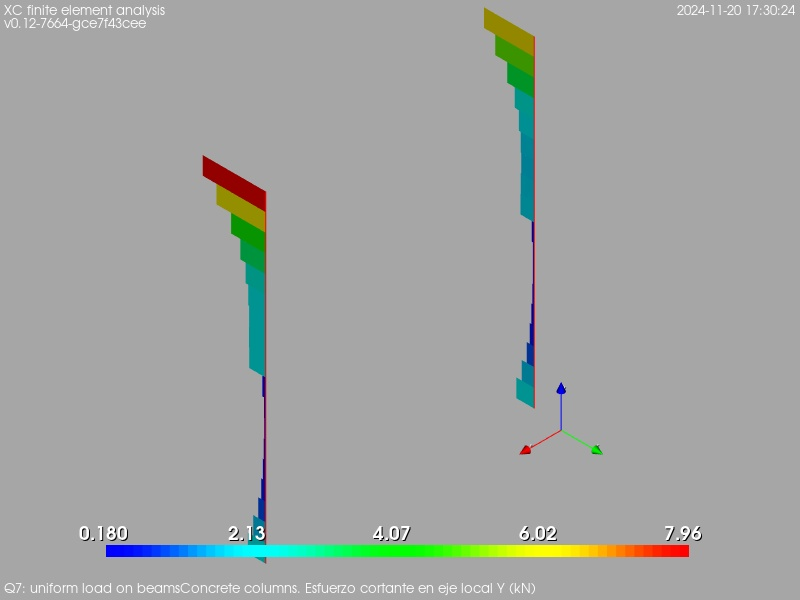
\includegraphics[width=\linewidth]{results/graphics/resSimplLC/qunifBeamscolumnZconcrVy.png}
\caption{Q7: uniform load on beamsConcrete columns. Esfuerzo cortante en eje local Y (kN)}
\label{qunifBeamscolumnZconcrVy}
\end{center}
\end{figure}
\begin{figure}[ht]
\begin{center}
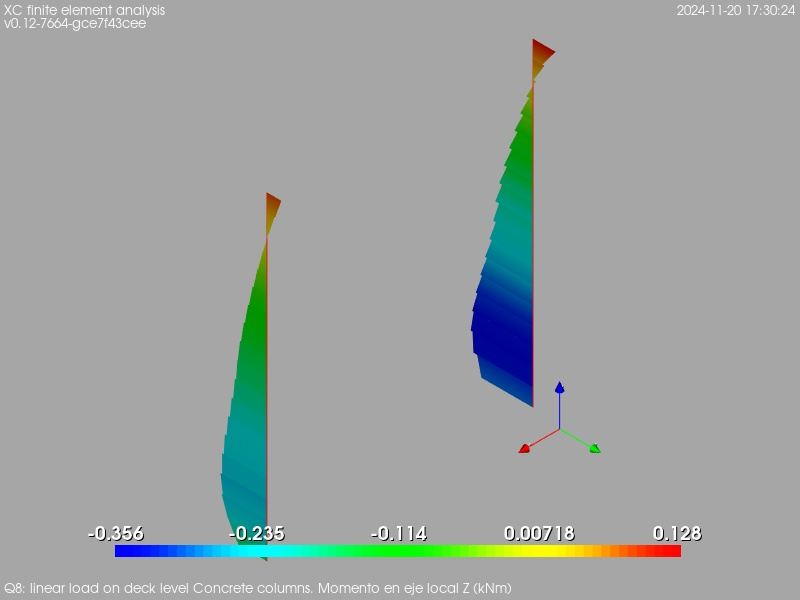
\includegraphics[width=\linewidth]{results/graphics/resSimplLC/qlinDeckcolumnZconcrMz.png}
\caption{Q8: linear load on deck level Concrete columns. Momento en eje local Z (kNm)}
\label{qlinDeckcolumnZconcrMz}
\end{center}
\end{figure}
\begin{figure}[ht]
\begin{center}
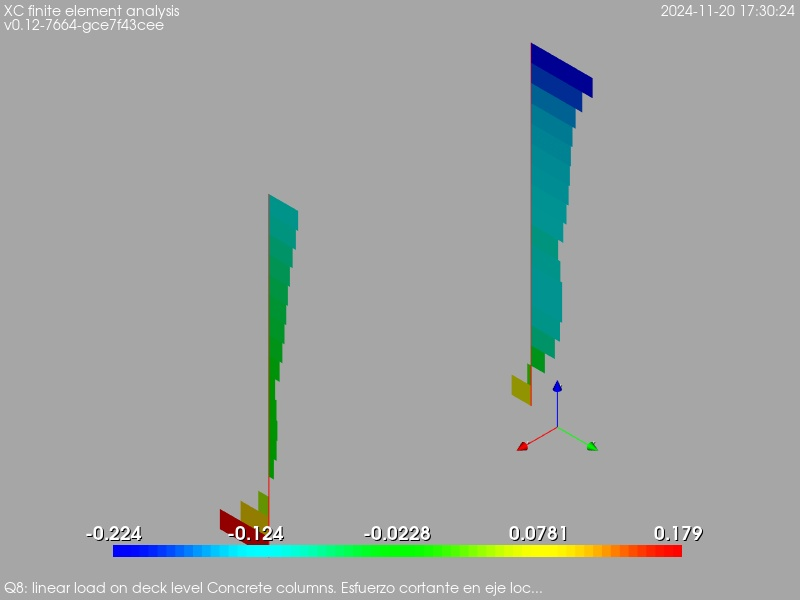
\includegraphics[width=\linewidth]{results/graphics/resSimplLC/qlinDeckcolumnZconcrVy.png}
\caption{Q8: linear load on deck level Concrete columns. Esfuerzo cortante en eje local Y (kN)}
\label{qlinDeckcolumnZconcrVy}
\end{center}
\end{figure}
\begin{figure}[ht]
\begin{center}
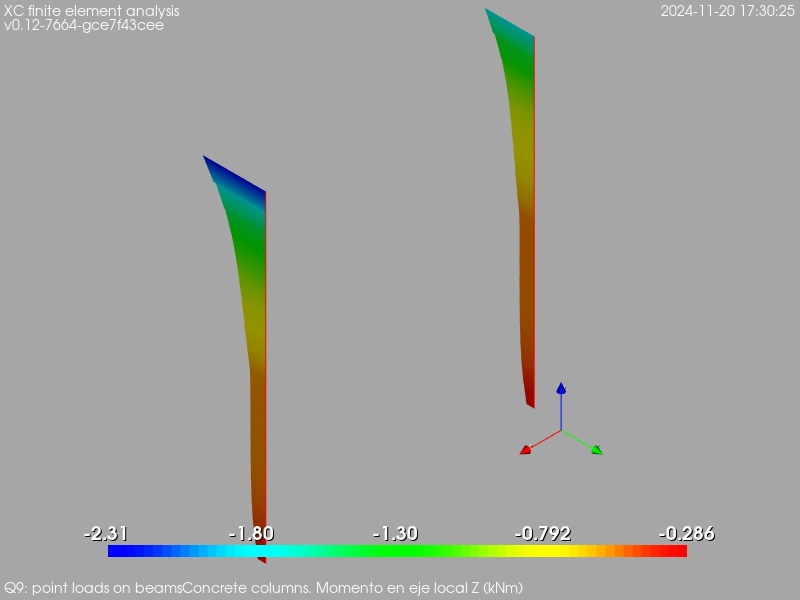
\includegraphics[width=\linewidth]{results/graphics/resSimplLC/QpntBeamscolumnZconcrMz.png}
\caption{Q9: point loads on beamsConcrete columns. Momento en eje local Z (kNm)}
\label{QpntBeamscolumnZconcrMz}
\end{center}
\end{figure}
\begin{figure}[ht]
\begin{center}
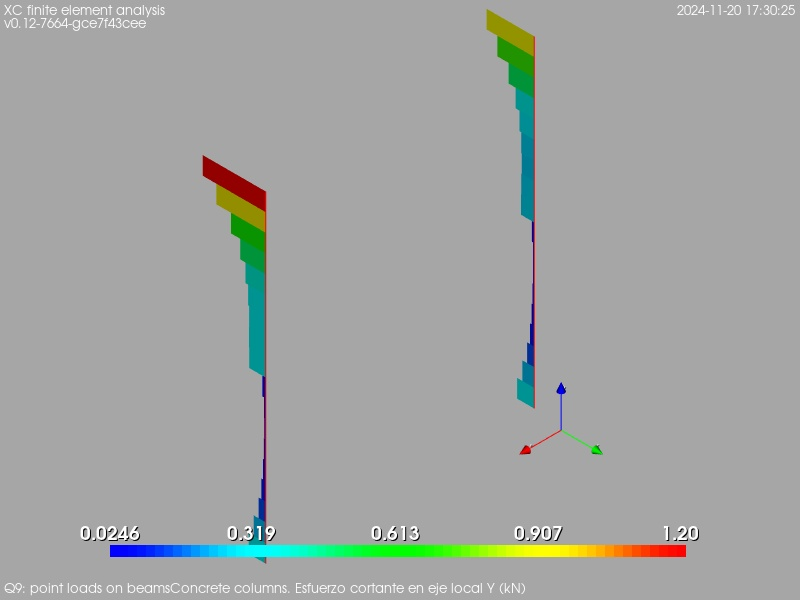
\includegraphics[width=\linewidth]{results/graphics/resSimplLC/QpntBeamscolumnZconcrVy.png}
\caption{Q9: point loads on beamsConcrete columns. Esfuerzo cortante en eje local Y (kN)}
\label{QpntBeamscolumnZconcrVy}
\end{center}
\end{figure}
\begin{figure}[ht]
\begin{center}
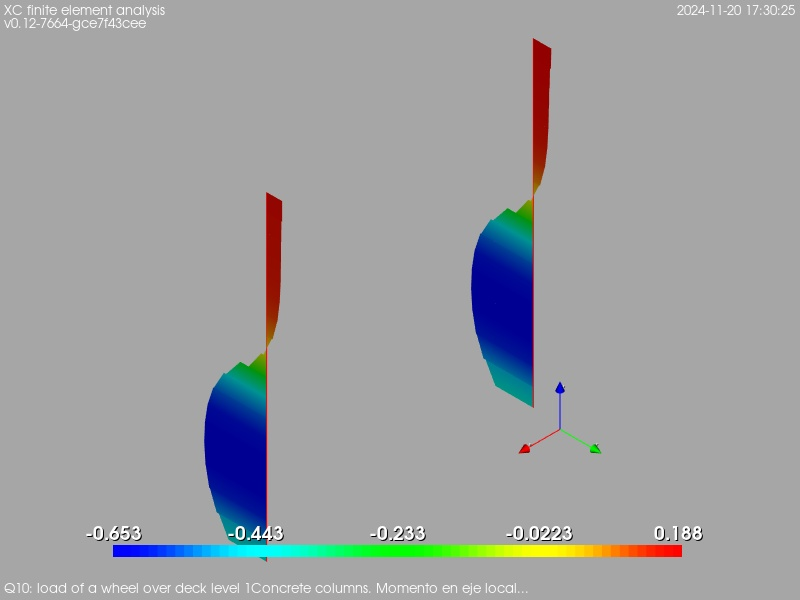
\includegraphics[width=\linewidth]{results/graphics/resSimplLC/QwheelDeck1columnZconcrMz.png}
\caption{Q10: load of a wheel over deck level 1Concrete columns. Momento en eje local Z (kNm)}
\label{QwheelDeck1columnZconcrMz}
\end{center}
\end{figure}
\begin{figure}[ht]
\begin{center}
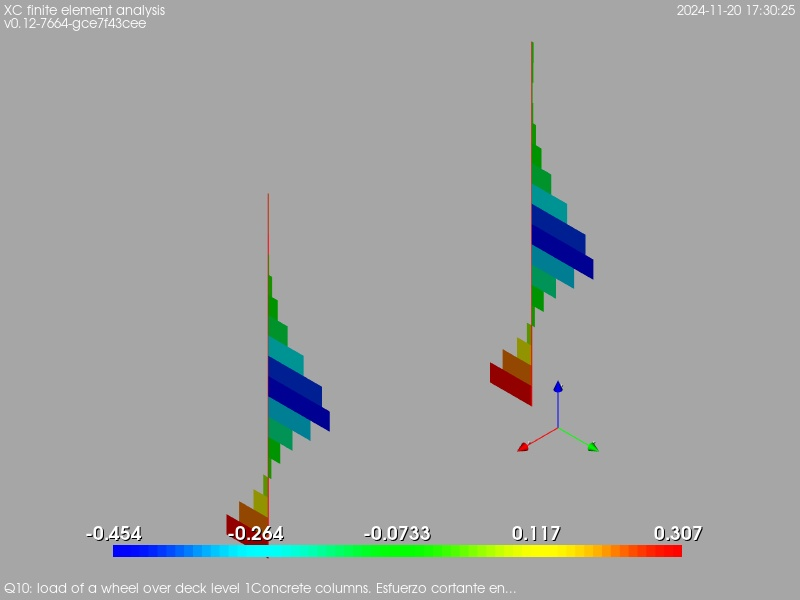
\includegraphics[width=\linewidth]{results/graphics/resSimplLC/QwheelDeck1columnZconcrVy.png}
\caption{Q10: load of a wheel over deck level 1Concrete columns. Esfuerzo cortante en eje local Y (kN)}
\label{QwheelDeck1columnZconcrVy}
\end{center}
\end{figure}
\begin{figure}[ht]
\begin{center}
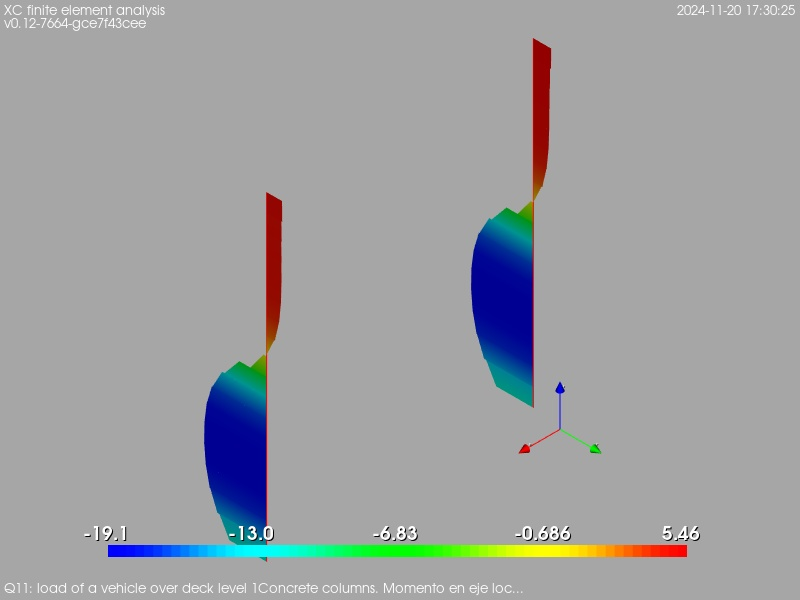
\includegraphics[width=\linewidth]{results/graphics/resSimplLC/QvehicleDeck1columnZconcrMz.png}
\caption{Q11: load of a vehicle over deck level 1Concrete columns. Momento en eje local Z (kNm)}
\label{QvehicleDeck1columnZconcrMz}
\end{center}
\end{figure}
\begin{figure}[ht]
\begin{center}
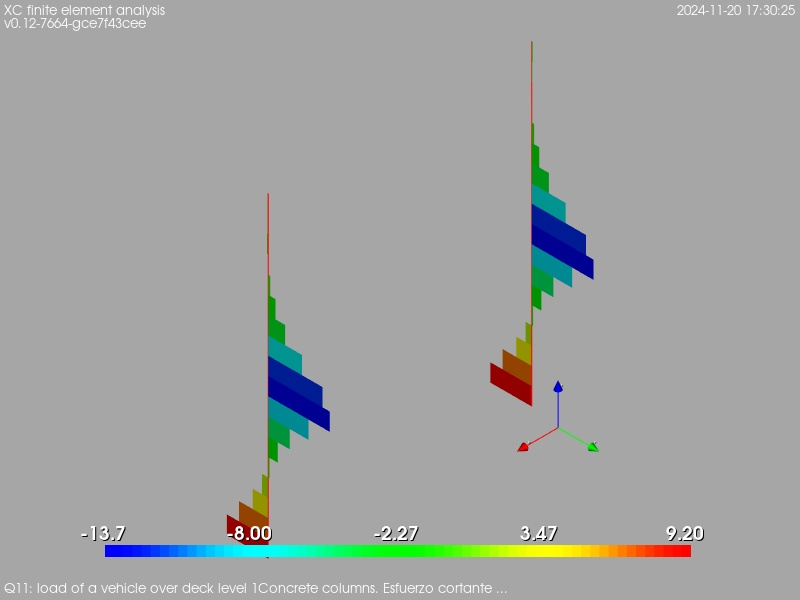
\includegraphics[width=\linewidth]{results/graphics/resSimplLC/QvehicleDeck1columnZconcrVy.png}
\caption{Q11: load of a vehicle over deck level 1Concrete columns. Esfuerzo cortante en eje local Y (kN)}
\label{QvehicleDeck1columnZconcrVy}
\end{center}
\end{figure}
\begin{figure}[ht]
\begin{center}
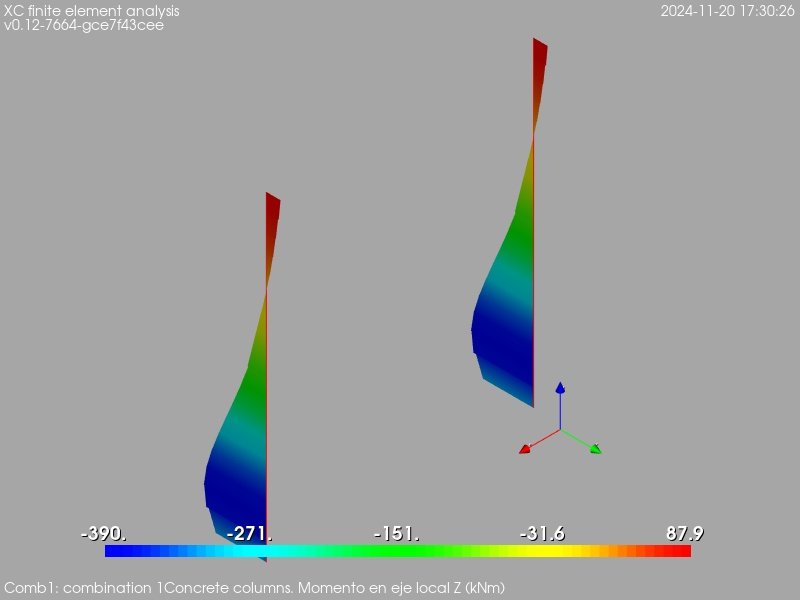
\includegraphics[width=\linewidth]{results/graphics/resSimplLC/LS1columnZconcrMz.png}
\caption{Comb1: combination 1Concrete columns. Momento en eje local Z (kNm)}
\label{LS1columnZconcrMz}
\end{center}
\end{figure}
\begin{figure}[ht]
\begin{center}
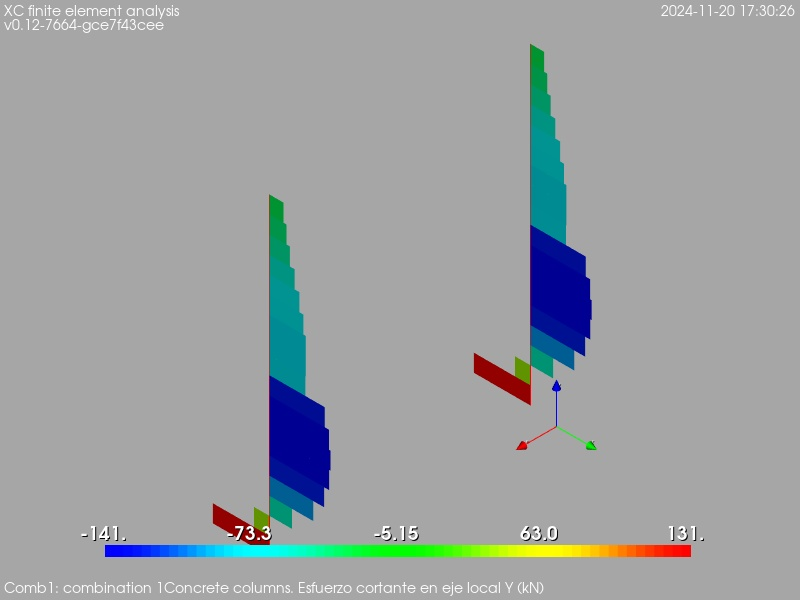
\includegraphics[width=\linewidth]{results/graphics/resSimplLC/LS1columnZconcrVy.png}
\caption{Comb1: combination 1Concrete columns. Esfuerzo cortante en eje local Y (kN)}
\label{LS1columnZconcrVy}
\end{center}
\end{figure}
\begin{figure}[ht]
\begin{center}
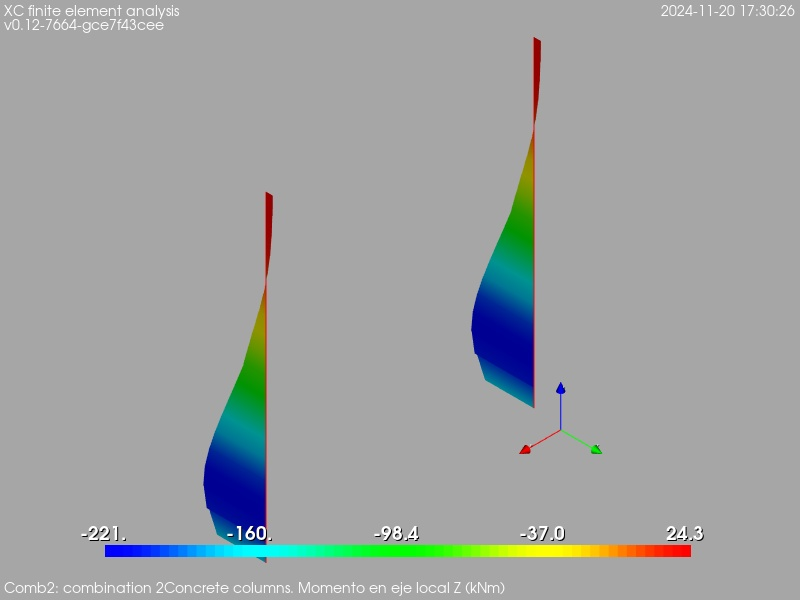
\includegraphics[width=\linewidth]{results/graphics/resSimplLC/LS2columnZconcrMz.png}
\caption{Comb2: combination 2Concrete columns. Momento en eje local Z (kNm)}
\label{LS2columnZconcrMz}
\end{center}
\end{figure}
\begin{figure}[ht]
\begin{center}
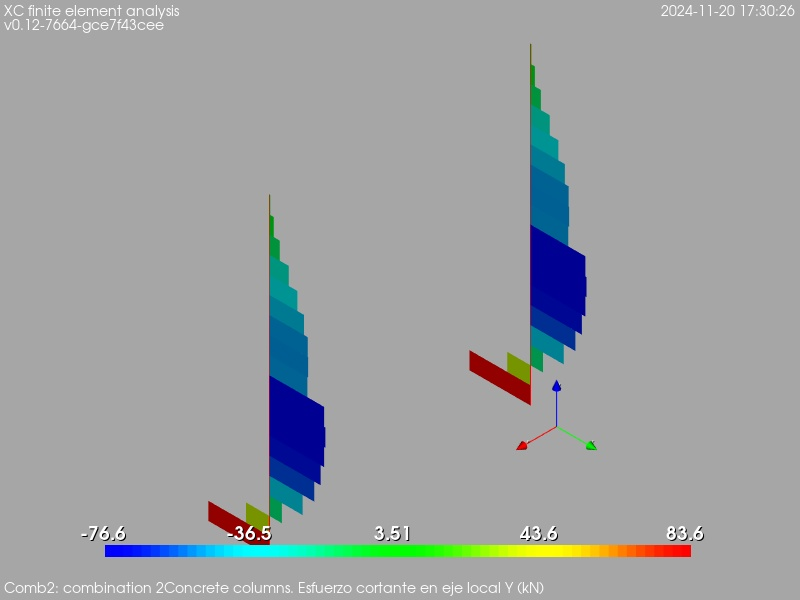
\includegraphics[width=\linewidth]{results/graphics/resSimplLC/LS2columnZconcrVy.png}
\caption{Comb2: combination 2Concrete columns. Esfuerzo cortante en eje local Y (kN)}
\label{LS2columnZconcrVy}
\end{center}
\end{figure}
\clearpage 
